\documentclass[tikz,border=2pt]{standalone}
\usepackage{tikz}
\usetikzlibrary{shapes.arrows}
\begin{document}
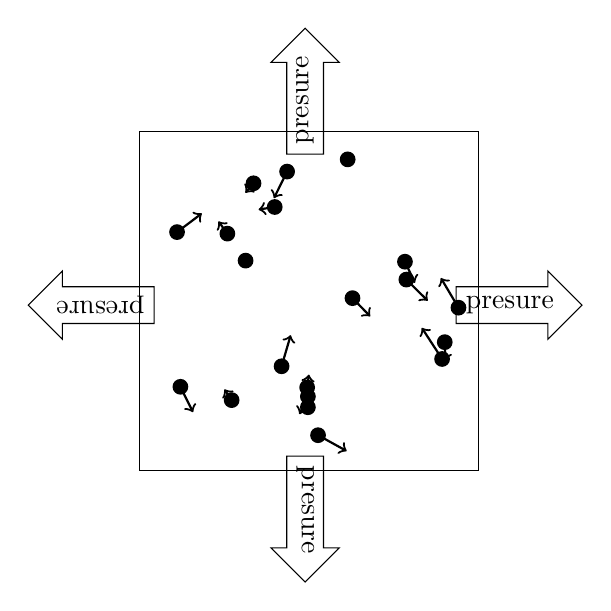
\begin{tikzpicture}[scale=2.0]

	\draw (-1.05, -1.05) rectangle (1.1,1.1);
	\foreach[evaluate={\a=rand; \b=rand;\c=rand;\d=rand;}] \x in {1,...,20}{
		\fill (\a, \b) circle [radius=0.05];
		\draw[->,thick] (\a, \b) -- (\a+\c*0.2, \b+\d*0.2);
	}
\node[draw, single arrow, minimum height=10mm, minimum width=3mm,
              single arrow head extend=2mm, rotate=90] at (0.0,1.3) {presure};
\node[draw, single arrow, minimum height=10mm, minimum width=3mm,
              single arrow head extend=2mm, rotate=-90] at (0.0,-1.3) {presure};
\node[draw, single arrow, minimum height=10mm, minimum width=3mm,
              single arrow head extend=2mm, rotate=0] at (1.3,0.0) {presure};
\node[draw, single arrow, minimum height=10mm, minimum width=3mm,
              single arrow head extend=2mm, rotate=180] at (-1.3,0.0) {presure};

\end{tikzpicture}
\end{document}
